\chapter{توصیف معماری سیستم}
\noindent
\textbf{
	\textit{
		تشریح اینترفیس‌های سیستم، کلاک‌ها و نحوهٔ راه‌اندازی سیستم، دیاگرام بلوکی سخت‌افزار، ساختار درختی سیستم و توصیف ماژول‌های سخت‌افزار 
	}
}
\pagebreak

\section{ اینترفیس‌های سیستم}
در ابتدا به صورت خلاصه اینترفیس‌های سیستم سخت‌افزاری الگوریتم Skein بیان می‌شود، اینترفیس یک سیستم شامل ورودی‌ها و خروجی‌ها و مشخصات ایشان است. 
\subsection{ورودی‌ها}
ورودی‌ها کد verilog الگوریتم Skein به شرح زیر اند.
\begin{itemize}
	\item
	      \textbf{clk}\\
	      ورودی کلاک سیستم است که با آن سیستم کار خود را به صورت ترتیبی 
	      \footnote{\lr{Sequential}}
	      انجام می‌دهد، فرکانس کلاک با توجه به نحوهٔ پیاده‌سازی سخت‌افزاری و نتایج حاصل از سنتز تعیین می‌شود.
	\item
	      \textbf{\lr{midstate}}\\
	      ورودی‌ای ۵۱۲ بیتی برای الگوریتم
	      \lr{Skein-512}
	      است که حالت میانی در هش را معلوم می‌کند.
	\item
	      \textbf{nonce}\\
	      nonce مقداری دلخواه است که برای به حداکثر رساندن تصادفی  و غیرقابل شکستن بودن هش 
	      در محاسبه هش استفاده می‌شود، این مقدار می‌تواند عددی دلخواه باشد. در الگوریتم 
	      \lr{Skein-512}
	      اندازهٔ این ورودی ۳۲ بیت به اندازه طول عدد در Integer گرفته شده است.
	\item
	      \textbf{data}\\
	      ورودی اصلی‌ست که باید هش آن محاسبه شود، در کد verilog داده شده اندازه این ورودی ۹۶ بیت در نظر گرفته شده است. 
\end{itemize}

\subsection{خروجی}
تنها خروجی سیستم مقدار هش در output است که ۵۱۲ بیت طول دارد.
(الگوریتم مورد بحث 
\lr{Skein-512}
است)

\section{کلاک‌ها و نحوهٔ راه‌اندازی سیستم}
این سیستم فقط از یک کلاک استفاده می‌کند و برای راه‌اندازی سیستم انجام کارهای زیر ضروری‌ست.
\begin{enumerate}
	\item
	      وصل کردن کلاک با فرکانس مناسب به سیستم
	\item
	      اعمال ریست‌ کلی بر سیستم
	      \footnote{\lr{Global Reset}}
	\item 
	      تعیین ورودی‌های اولیه 
	\item 
	      راه‌اندازی سیستم 
\end{enumerate}


\section{دیاگرام بلوکی سخت‌افزار}
دیاگرام بلوکی کلی سخت‌افزار در شکل 
\ref{block_diagram}
آمده است. 

\begin{figure}
	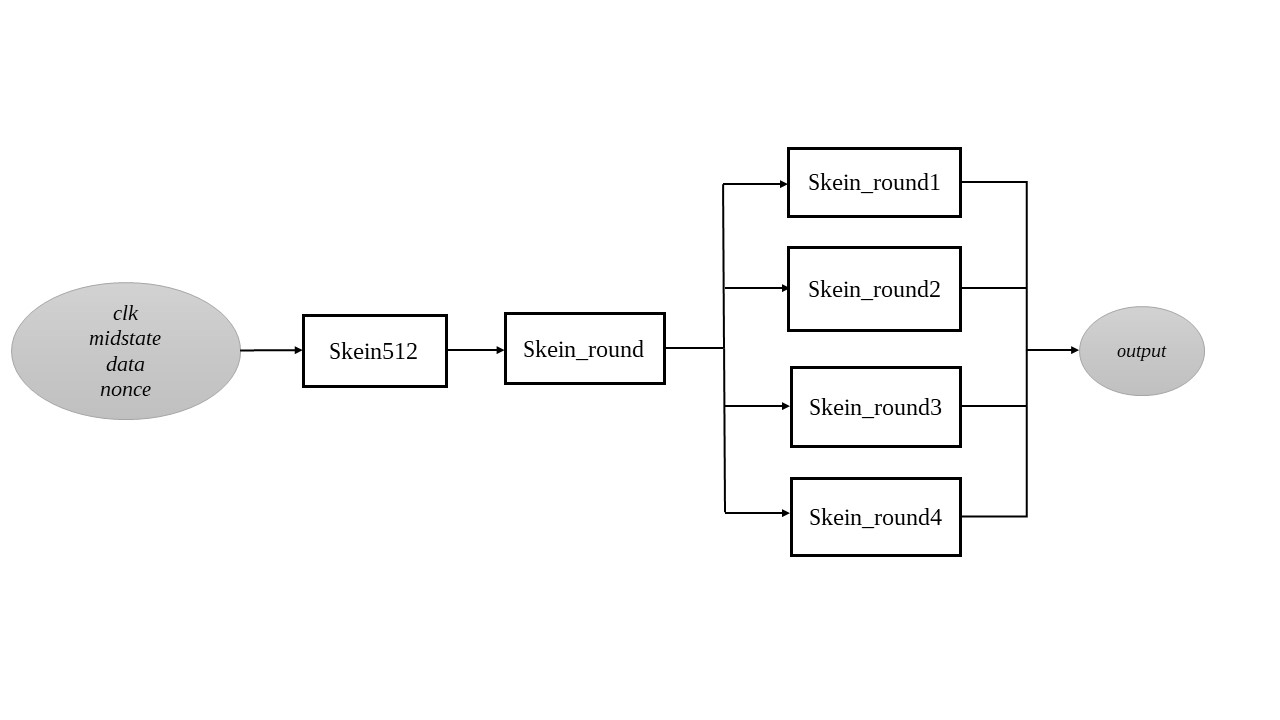
\includegraphics[width = \textwidth]{figs/DescriptionOfSystem/block_diagram.jpg}
	\caption{دیاگرام بلوکی سخت‌افزار}
	\label{block_diagram}
\end{figure}

\section{توصیف ماژول‌های سخت‌افزار}
\subsection{\lr{Skein-512}}
ابتدا تعدادی reg و wire گرفته شده است.
دو reg به نام های$ phase\_d$ و $phase\_q $تعریف شده اند که یک‌بیتی اند و مقدار صفر به آنها داده شده است.\\
دو عبارت assign در کد وجود دارد.

\begin{enumerate}
	\item در reg 32 بیتی با نام $nonce\_le$ که در خطوط بالاتر تعریف شده است مقادیر $nonce$ (که ورودی 32 بیتی ماژول هستند) به صورت 8 بیت – 8 بیت و به صورت برعکس ذخیره می‌شوند. یعنی به طور مثال 8 بیت کم ارزش\  $nonce$در 8 بیت پرارزش $nonce\_le$ ذخیره شده اند. (خط 55)lk
	      
	\item در reg 32 بیتی با نام $nonce2\_le$ که در خطوط بالاتر تعریف شده است مقادیر $nonce2$ (که برعکس $nonce$، ورودی ماژول نیست و خود در خطوط بالاتر به صورت یک reg 32 بیتی تعریف شده است و در واقع در حال حاضر مقداری را به خود اختصاص نداده است) به صورت 8 بیت – 8 بیت و به صورت برعکس ذخیره می‌شوند. یعنی به طور مثال 8 بیت کم ارزش\  $nonce2$در 8 بیت پرارزش  $nonce2\_le$ ذخیره شده اند. (خط 56)
\end{enumerate}

یک عبارت assign طویل مربوط به hash دیده می‌شود:

\begin{itemize}
	\item
	      در این عبارت بیت‌های reg ی به نام
	      h\_q 
	      که 512 بیت دارد و در خطوط بالاتر تعریف شده است، به بیت های خروجی hash اساین می‌شود.
	\item
	      64 مجموعه 8 بیتی از $h\_q$ به بیت های hash اساین می‌شود که نظم این مقداردهی در زیر توضیح داده می‌شود. در این توضیحات hash را به ترتیب از پرارزش‌ترین بیت شروع به پر کردن میکنیم.
	\item
	      پرارزش‌ترین بیت‌های hash با بیت های $463$ تا $456$ پر شده است. (یعنی پرارزش ترین بیت hash با بیت $463$ ام $h\_q$ پر شده است و به همین ترتیب)
	\item
	      مجموعه بعدی 8 تایی از$464$ تا $471$ هستند که در دومین 8 تایی با ارزش hash قرار می‌گیرند.
	\item
	      این روند تا هشتمین 8 بیت ارزشمند hash ادامه پیدا میکند جایی که در این جایگاه مجموعه $[511:504]$ از $h\_q$ جای میگیرد. (تا اینجا نظم داشتیم)
	\item
	      نهمین 8 بیت ارزشمند hash توسط بیت های $[391:384]$ از $h\_q$ پر میشوند.
	\item
	      این روند ادامه پیدا میکند (یعنی دهمین 8 بیت ارزشمند با $[399:392]$ پر میشوند).
	      تا 16امین 8 بیت ارزشمند hash که با مجموعه $[447:440]$ پر شده اند.
	\item
	      17امین 8 بیت ارزشمند با مجموعه $[327:320]$ پر میشود.
	\item2
	      این روند مانند قبل به صورت صعودی ادامه پیدا خواهد کرد تا به 25 امین مجموعه 8 بیتی برسیم.
	      
\end{itemize}

\textit{\textbf{درواقع هر 8 بار که مجموعه بیت های 8 بیتی را assign میکنیم، یک بی‌نظمی داریم.
}}
\begin{itemize}
	\item
	      25 امین 8 بیتی hash با بیت های $[263:256]$ پر میشود.
	\item
	      دوباره روند سابق و صعودی را داریم تا به 33 امین assignment برسیم.
	\item
	      33 امین 8 بیتی hash با بیت های $[199:192]$
	      
\end{itemize}

\textit{\textbf{هر بار بی‌نظمی داریم بازه جدید بعد از بی نظمی 120 واحد کمتر از بازه قبلی خواهد بود مثلا 32 امین 8بیت پرارزش hash با بیت های $[319:312] $پر شده اند که 120 واحد از بازه ای که برای 33امین 8 بیت ارزشمند hash اختصاص داده میشود بیشتر است. (در بالا 33امین نوشته شده است)}}

\begin{itemize}
	\item
	      باز 8 مجموعه که به صورت صعودی پیش برویم به 40 امین 8بیت میرسیم که طبق نظم با بیت های $[255:248]$ پر شده است و 41امین 8 بیتی با بازه $[135:128]$ پر شده است.
	\item
	      باز 8 مجموعه که به صورت صعودی پیش برویم به 48 امین 8بیت میرسیم که طبق نظم با بیت های $[191:184]$ پر شده است و 49امین 8 بیتی با بازه $[71:64]$ پر شده است.
	\item
	      باز 8 مجموعه که به صورت صعودی پیش برویم به 56 امین 8بیت میرسیم که طبق نظم با بیت های $[127:120]$ پر شده است و 57امین 8 بیتی با بازه $[7:0]$ پر شده است.
	\item
	      از 57 امین مجموعه 8 تایی با ارزش hash تا آخرین مجموعه باارزش hash (64 امین) نیز به صورت صعودی و طبق نظم پیش میرود. (خط 121)
	      
\end{itemize}

بعد از خطوط assignment، 18 instance از ماژول skein\_round گرفته شده است.
این instance ها را از 
$00$
تا
$0H$
نام گذاری کردیم (نامگذاری در مبنای بالاتر از 10 شده است)

\subsubsection{
	ورودی skein\_round ها
}
\begin{itemize}
	\item
	      \textbf{کلاک}
	      که همه به کلاک سیستم متصل اند.
	\item
	      \textbf{Round}
	      رجیستر 32 بیتی که به ترتیب ورودی 0 تا 17 به هر اینستنس داده شده است.
	\item
	      \textbf{$p$}
	      رجیستر 512 بیتی – که اینستنس شماره $01$ تا $0H$ به ترتیب $p01$ تا $p0H$ وصل شده است. به اینستنس شماره $00$ هم $p00\_q$ وصل شده است.
	\item
	      \textbf{$H$}
	      رجیستر 576 بیتی – که اینستنس شماره $01$ تا $0H $به ترتیب $h01$ تا $h0H$ وصل شده است. به اینستنس شماره $00$ هم $h00\_q$ وصل شده است.
	\item
	      \textbf{$T0$}
	      رجیستر 64 بیتی –   که از اینستنس شماره $00$ تا $0H$ به ترتیب این دنباله 3 تایی وصل شده است:$ t0\_q, t1\_q , t2\_q $این دنباله 3 جمله ای به ترتیب تکرار میشود.
	\item
	      \textbf{$T1$}
	      رجیستر 64 بیتی – دقیقا مثل $T0$ با این تفاوت که دنباله 3 تایی$ t1\_q ، t2\_q و t0\_q $به ای شکل است.
	\item
	      \textbf{$P0$}
	      رجیستر 512 بیتی- که اینستنس شماره $00$ تا $0H$به ترتیب $o00$ تا $o0H$ وصل شده است. 
	\item
	      \textbf{$H0$}
	      رجیستر 576 بیتی- که اینستنس شماره $00$ تا $0H $به ترتیب $ho00 $تا $ho0H$ وصل شده است. خط(141)
	      
\end{itemize}
\textit{\textbf{
	در ادامه یک always بلاک داریم که حساس به تغییرات همه چیز است. (خط 143)
	در این بلاک متغیر هایی که در انتها
	\_d
دارند مقداردهی میشوند.}}
ابتدا phase\_d مقدار not متغیر phase\_q را به خود اختصاص میدهد.
\begin{itemize}
	\item
	      \textbf{اگر phase\_q یک باشد}
	      \begin{itemize}
	      	\item
	      	      مقداردهی به $p00\_d$ (512 بیتی): 64 بیت کم ارزش ( $[63:0]$) از data در 64 بیت پرارزش $p00\_d$ قرار میگیرد. سپس در 32 بیت بعدی $p00\_d$ (از چپ) عینا nonce\_le قرار داده میشود. سپس 32 بیت باقیمانده از $data ([95:64])$ طبق روند قرار داده میشود. باقی بیت های این رجیستر هم با صفر پر میشوند $(384’d0)$ – (خط 148)
	      	\item
	      	      مقداردهی به$ h00\_d$ (576 بیتی): در 64 بیت کم ارزش این reg، مقدار صفر قرار داده میشود و باقی بیت ها دقیقا به midstate (ورودی 512 بیتی) متصل میشوند.
	      	\item
	      	      مقداردهی به$ t0\_d$ (64 بیتی) : $h0000000000000050$
	      	\item
	      	      مقداردهی به$ t1\_d$ (64 بیتی) : $hb000000000000000$
	      	\item
	      	      مقداردهی به $t2\_d$ (64 بیتی) : $hb000000000000050$
	      	\item
	      	      h\_d هم مقدار h\_q را به خود میگیرد.
	      \end{itemize}
	\item
\textbf{	      اگر phase\_q صفر باشد
}	      \begin{itemize}
	      	\item
	      	      مقداردهی به $p00\_d$ (512 بیتی): این reg با صفر پر میشود.
	      	\item
	      	      مقداردهی به $h00\_d$ (576 بیتی):
	      	      \begin{itemize}
	      	      	\item
	      	      	      بیت های $[575:512]$:	
	      	      	      	$data[63:0] \textasciicircum ( oH[511:448] + hH[575:512])$
	      	      	\item
	      	      	      بیت های $[511:448]$: 	{ nonce2\_le, $data[95:64]$ } \textasciicircum ( $oH[447:384] + hH[511:448]$)
	      	      	\item
	      	      	      بیت های $[447:384]$:  $	oH[383:320] + hH[447:384]$
	      	      	\item
	      	      	      بیت های $[383:320]$:$	oH[319:256] + hH[383:320]$
	      	      	\item
	      	      	      بیت های $[319:256]$:$	oH[255:192] + hH[319:256]$
	      	      	\item
	      	      	      بیت های $[255:192]$:
	      	      	      $	oH[191:128] + hH[255:192] + 
	      	      	      64'h0000000000000050$
	      	      	\item
	      	      	      بیت های $[191:128]$:	
	      	      	      $oH[127: 64] + hH[191:128] + 64'hb000000000000000$
	      	      	\item
	      	      	      بیت های $[127:64]$:
	      	      	  $    	oH[ 63:  0] + hH[127: 64] + 18$
	      	      \end{itemize}
	      	\item
	      	      مقداردهی به$ t0\_d$ (64 بیتی) : $h0000000000000008$
	      	\item
	      	      مقداردهی به $t1\_d$ (64 بیتی) : $hFF00000000000000$
	      	\item
	      	      مقداردهی به $t2\_d$ (64 بیتی) : $hFF00000000000008$
	      	\item
	      	      مقداردهی به $h\_d$ (512 بیتی):
	      	      \begin{itemize}
	      	      	\item
	      	      	      بیت های $[511:448]$:
	      	      	      $ 	o0H[511:448] + ho0H[575:512]$
      	      	    \item
	      	      	      بیت های $[447:384]$:  
	      	      	      	$o0H[447:384] + ho0H[511:448]$
	      	      	\item
	      	      	      بیت های $[383:320]$:
	      	      	      $	o0H[383:320] + ho0H[447:384]$
	      	      	\item
	      	      	      بیت های $[319:256]$:
	      	      	      $	o0H[319:256] + ho0H[383:320]$
	      	      	\item
	      	      	      بیت های $[255:192]$:
	      	      	      $	o0H[255:192] + ho0H[319:256]$
	      	      	\item
	      	      	      بیت های $[191:128]$:	
	      	      	      $o0H[191:128] + ho0H[255:192] + 64'h0000000000000008$
	      	      	\item
	      	      	      بیت های $[127:64]$:	
	      	      	      $o0H[127: 64] + ho0H[191:128] + 64'hFF00000000000000$
	      	      	\item
	      	      	      بیت های $[63:0]$:	
	      	      	      $	o0H[ 63:  0] + ho0H[127: 64] + 18$
	      	      	 
	      	      \end{itemize}
	      \end{itemize}
\end{itemize}
\textit{
	\textbf{نظم مناسبی دیده میشود به این شکل که به ترتیب 64 بیت پرارزش h\_d با مجموع 64 بیت پرارزش $o0H$ و 64 بیت پرارزش $ho0H$ پر میشود. به جز 3 مورد آخر که با اعدادی ثابت جمع میشوند.
}}

\textit{\textbf{Always بلاک دوم فقط به لبه مثبت کلاک حساس است. (خط 211)
	(عموما متغیر های \_q، مقادیر متناظر \_d را به خود میگیرند) }}
\begin{itemize}
	\item
	      $hH$ مقدار $ho0H$ را به خود میگیرد.
	\item
	      $oH$ مقدار $o0H$ را به خود میگیرد.
	\item
	      $phase\_q$ مقدار $phase\_d$ را به خود میگیرد.
	\item
	      $h\_q$ مقدار $h\_d$ را به خود میگیرد.
	\item
	      $t0\_q$ مقدار $t0\_d$ را به خود میگیرد.
	\item
	      $t1\_q$ مقدار $t1\_d$ را به خود میگیرد.
	\item
	      $t2\_q$ مقدار $t2\_d$ را به خود میگیرد.
	\item
	      در ادامه مجموعه ای از مقدار دهی ها را مربوط به reg های $p0x$ (x منظور از 1  تا H) و $h0x$ (x منظور از   1  تا H) داریم. (خط 226 تا 261)
	\item
	      $h0x$ ها: مقدار $ho0y$ را میگیرند با این تفاوت که y از x یک واحد کمتر است. (به طور مثال $h01$ مقدار $ho00$ را به خود میگیرد)
	\item
	      $p0x$  ها: مقدار $o0y$ را میگیرند با این تفاوت که y از x یک واحد کمتر است. (به طور مثال $h01$ مقدار $o00$ را به خود میگیرد)
	\item
	      $p00\_q$ مقدار $p00\_d$ را میگیرد.
	\item
	      $h00\_q$ مقدار $h00\_d$ را میگیرد.
	\item
	      $nonce2$ هم که در ابتدای فایل مقداری مجهول داشت اینجا مقدار $nonce$ (ورودی)  منهای 32$’d54$
	       را میگیرد.
\end{itemize}